\documentclass[11pt]{article}

\usepackage[utf8]{inputenc}
\usepackage[T1]{fontenc}
\usepackage{lmodern}
\usepackage[margin=1in]{geometry}
\usepackage{amsmath,amssymb}
\usepackage{booktabs}
\usepackage{float}
\usepackage{tabularx}
\usepackage{array}
\usepackage{enumitem}
\usepackage{fvextra}
\usepackage{newunicodechar}
\usepackage{tikz}
\usetikzlibrary{arrows.meta,positioning,fit,backgrounds}
\usepackage[numbers,sort&compress]{natbib}
\usepackage[hidelinks]{hyperref}

\newunicodechar{≠}{\ensuremath{\neq}}
\newunicodechar{∧}{\ensuremath{\wedge}}
\newunicodechar{→}{\ensuremath{\to}}
\newunicodechar{∀}{\ensuremath{\forall}}
\newunicodechar{¬}{\ensuremath{\neg}}
\newunicodechar{∃}{\ensuremath{\exists}}
\newunicodechar{≤}{\ensuremath{\le}}
\newunicodechar{∈}{\ensuremath{\in}}

\newcommand{\code}[1]{\texttt{#1}}
\newcommand{\lean}[1]{\texttt{#1}}

\title{CogLean: Towards a Machine-Checkable Library of Cognitive Theory}
\author{Jeff Shrager}
\date{Draft, November 2026}

\begin{document}
\sloppy
\maketitle

\begin{center}
\fbox{\parbox{0.9\linewidth}{\centering\large\textbf{Draft for Comment}\footnotemark}}
\end{center}

\footnotetext{This is a working draft. I welcome corrections,
  constructive challenges, and especially proposals for
  collaboration. Email me: \texttt{jshrager@gmail.com}.}
\medskip

\begin{abstract}
CogLean is a library of cognitive theory expressed in the Lean
programming language and proof assistant, in which the definitions
that run as models are the same objects that theorems are about. Its
premise is that once we write down what we already believe about a
cognitive theory with mathematical precision, we can discover things
about that theory that we did not know. This paper is an invitation
to cognitive scientists, and assumes no knowledge of Lean. It asks
four questions a cognitive scientist might ask of such a library and
answers each with one short demonstration. Does a theory entail what
its authors said? Siegler and Shrager's 1984 model of strategy choice
is checked: its ``nonintuitive prediction'' is proved, and a claim in
the same chapter turns out to need a condition the chapter does not
state, a condition the formalization found. Can a theory be shown unable to
produce a phenomenon? Collins and Quillian's hierarchical network can
never show a typicality effect, for any network, while a feature
comparison model can. Do independently formalized theories compose?
EPAM, the strategy-choice model and a problem solver compose into a
model of three-digit addition, a pattern of confident errors is proved
for the composition and for every memory satisfying three laws, a
simplified ACT-R memory reaches the pattern by another route, and the
two explanations differ on an experiment nobody has run, which the
comparison produced rather than presupposed. Can theories
be compared by what they entail rather than how they fit? A memory
theory matrix classifies four formalized memory families against six
laws of retrieval, every verdict a theorem. What these discoveries
establish is about the theories, not directly about people; their
psychological significance still turns on empirical assumptions. The
goal is to grow CogLean into a Mathlib-like repository of
machine-checkable cognitive theory, in which such results accumulate,
and the paper closes with what each kind of cognitive scientist could
contribute to it.
\end{abstract}

\section{Four questions}
\label{sec:intro}

Suppose a cognitive theory were written down precisely enough that a
machine could check what follows from it. What would we want to ask?
Not, in the first place, whether the theory fits a data set; we have
good tools for that. The questions I have in mind are the ones that
come up when theories are discussed rather than fitted. Does the
theory, as written, actually entail the predictions its authors drew
from it? Is there a phenomenon it \emph{cannot} produce, whatever its
parameters? When two theories explain the same phenomenon, do they
explain it for the same reasons, and what observation would tell them
apart? And can theories be compared by what they entail, rather than
by how well each can be made to fit? Behind all of these is one idea.
If we can write down what we already believe about a theory with
mathematical precision, then the theory becomes something we can
reason about mechanically, and we can discover consequences,
limitations and unstated assumptions that we did not know were there,
and perhaps would not have found otherwise. Formalization is the
necessary first step; discovery is the payoff.

These questions are old, and cognitive scientists have always answered
them by argument, by simulation, and sometimes by mathematics. What
has been missing is a place where the answers accumulate. Allen Newell
famously complained that cognitive science was collecting
independent phenomena and theories (``playing twenty questions with
nature'') instead of assembling unified understandings of cognition
\citep{newell1973}. Cognitive architectures such as Soar
\citep{laird1987,laird2012} and ACT-R \citep{anderson2007}, and the
Common Model of Cognition \citep{laird2017}, are direct responses to
Newell's complaint. Although such architectures bring together
multiple mechanisms to explain multiple phenomena, they are usually
rendered either as computational models (simulations), or as
principles asserted about such models. Cognitive principles have been
stated in formalisms that can be checked computationally
\citep{milnes1992,cooper1996,stewart2007,gall2018,langenfeld2019}, but
these efforts have proceeded model by model, and there has been no
shared, cumulative library in which machine-checked results about
mechanisms accumulate and stay aligned with the models that run.

The Lean proof assistant \citep{demoura2021} makes such a library
possible. Lean is, at the same time, an efficient functional
programming language with an unusually rich type system, and a system
for stating and mechanically checking proofs, so \emph{theorems are
about the same code that runs}. Lean has been used, increasingly with
the help of AI systems, to formalize and check large bodies of
mathematics \citep{mathlib2020}. CogLean applies this model to
cognitive science, seeking to align computational models of cognitive
mechanisms with assertions about those models and the phenomena they
produce. One caution belongs here, at the start. The checker
establishes that conclusions follow from premises. It does not
establish that the premises are true of people; that remains the
business of experiment. What is discovered this way is discovered
about the theories, and its psychological significance depends on
empirical assumptions that the paper tries to keep in view. What the
checker adds is that the entailments, once checked, stay checked, and
can be built upon.

This paper is an invitation, not a tutorial. No Lean is needed to read
it; where a few lines of Lean appear, they are there to show what a
theorem looks like, and each is paraphrased in English beside it.
After a short account of what CogLean is (Section~\ref{sec:clcl}), the
heart of the paper (Section~\ref{sec:demos}) takes the four questions
above in turn and answers each with one demonstration from the
library. The demonstrations are modest on purpose: a chapter checked,
an impossibility proved, a composition that works, a table of
theories against laws. Each is meant to show a kind of thing CogLean
can do, in a form that a reader could imagine doing with a theory of
their own. The Discussion (Section~\ref{sec:disc}) says what the four
answers have in common, and the paper ends (Section~\ref{sec:invite})
by saying what different kinds of cognitive scientists could
contribute.

One can approach CogLean from many directions. The most obvious, and
potentially the most useful, is for researchers working on cognitive
architectures to state their architectures' assertions in Lean. It
would also be useful for experimental psychologists to state phenomena
in CogLean and, where possible, the ``mid-level'' mechanisms they
propose for them. I leave the architectures to the architects, and the
phenomena to the psychologists. For historical and personal reasons,
the demonstrations here lean toward theories I know from the inside,
and toward the composition of mechanisms. I sincerely hope that readers
will \emph{not} simply follow my lead, but will invent their own ways
of using Lean in cognitive science, and in so doing extend the CogLean
repository and methodology.

\section{CogLean and CogLib}
\label{sec:clcl}

CogLean is the name I use for the overall project of applying Lean in
cognitive science. CogLib is a shared library of Lean
objects.\footnote{There should probably eventually be a division
between ``core'' and other sorts of objects.} CogLib follows the model
of Mathlib \citep{mathlib2020,demoura2021}. CogLib proposes no theory
of cognition, and complements cognitive architectures rather than
competing with them.

CogLean has four layers. Lean's core is the language and checker;
probabilities are exact rationals.\footnote{It is possible to develop
content that uses dense and infinite arithmetic by incorporating
Mathlib, but I've chosen not to do that here, as it is not needed.}
CogLib, the general library, holds representations, memories,
processes, an interface any memory can implement called a
``retriever'' (\lean{Cog.Retriever}: study an item; retrieve a
distribution over stored items), and theory-neutral phenomena and laws
with their theorems. A theory is a package that states its postulates
as choices of CogLib constructs, cites its sources, and proves its
phenomena and its mechanisms' laws. An application is a task model
built from theories and library mechanisms. Nothing in CogLib depends
upon any particular theory.

Two features make CogLib useful, not merely rigorous. First, in Lean a
definition is both a program and a mathematical object, so a model's
theorems are about the definitions that run; when a mechanism changes,
every explanation depending on it is rechecked. Second, because
mechanisms, phenomena and laws are shared, a result proved once is
available to every theory using the same constructs, and can be proved
for a whole class of mechanisms satisfying stated laws.

A few terms recur throughout, and a glossary (Appendix~\ref{app:glossary})
collects them. A \emph{mechanism} is a definition of a process, such
as how a net sorts an encoded stimulus. A \emph{phenomenon} is a
predicate over a task's outcomes that names no mechanism; it asserts
nothing until some mechanism is proved to satisfy it. A \emph{law} is a
property of a mechanism, such as that a studied item retrieves itself
for certain; in a theorem it is a hypothesis, not a Lean \code{axiom},
just as the group axioms are in Mathlib. A theorem's
\emph{conditions} are its other hypotheses: situational, unexplained
empirical premises, or matters of well-formedness. Every theorem in
this paper is fully proved, with no \code{sorry} (Lean's placeholder
for a missing proof), and every Lean name is given in full so that the
reader can find it in the repository.

\section{Four demonstrations}
\label{sec:demos}

\subsection{Does a theory entail what its authors said? The 1984 chapter}
\label{sec:doa}

In 1984, Bob Siegler and I proposed a model of how young children
choose between retrieving an arithmetic answer and working it out on
their fingers \citep{siegler1984}. The model's central claim was that
errors, solution times and overt strategy use ``are all functions of a
single variable: the distribution of associations between problems and
potential answers'' (p.~238). A child has, for each problem, a set of
associations of varying strength to possible answers. On a trial the
child sets a \emph{confidence criterion} and a \emph{search length},
samples an answer in proportion to its strength, states it if its
strength clears the criterion, and tries again up to the search
length; if nothing clears the criterion, the child falls back on
fingers, and then on counting. Stated answers are strengthened. The
chapter argued its predictions in prose and supported them with a
simulation. Forty years later, I wanted to know which of them actually
follow from the postulates.

CogLean's version of the model (\code{StrategyChoice/}) states the
six postulates of the chapter as choices from CogLib, each with its
page citation, and then proves its phenomena from them. Some of the
chapter's claims come out exactly as written. Retrieval is used with
probability $1-(1-R)^n$, where $R$ is the chance that a single search
clears the criterion and $n$ the search length
(\lean{SC.retrieval\_prob}). The share of errors among retrieval
trials is the wrong answers' share of the strength above the
criterion, whatever the search length
(\lean{SC.retrieval\_error\_share}). And the chapter's self-described
``nonintuitive prediction'' (p.~245), that the error rate on counting
trials does not depend on the associations at all, is a theorem:
\begin{Verbatim}[fontsize=\small]
theorem counting_error_share ... (p : Problem) (hT : total as s ≠ 0) :
    prob (trial as s bk cc n p) (countingWrong p) =
      prob (trial as s bk cc n p) isCounting *
        prob (count bk.qs bk.qd p.sum) (fun a => a != p.sum)
\end{Verbatim}
In words: on any problem, the probability of a wrong answer by counting
is the probability of counting at all, times the counting process's own
error rate on the correct sum. The associations, the criterion and the
search length appear on neither side of that product
(\lean{SC.counting\_error\_share}).

One claim did not survive as written. The chapter says that ``a peaked
distribution results in less frequent use of overt strategies''
(p.~245), which is intuitive: the more strength sits on the correct
answer, the more often retrieval should succeed. It is also, in
general, false. Moving strength from a wrong answer to the correct one
can \emph{raise} overt strategy use. The library's witness is small:
for $1+1$, with answers 2, 3 and 1 at strengths .38, .31 and .31,
moving one hundredth from the answer 3 to the correct answer 2 gives
.39, .30, .31, which is more peaked by any reasonable standard; yet the
predicted overt strategy use, averaged over the chapter's twelve
confidence criteria, rises from $7/12$ to $73/120$
(\lean{SC.peaking\_can\_raise\_overt\_use}). The reason is that the
wrong answer has dropped to the criterion .30 and so no longer clears
it, while the correct answer, at .39, was never going to clear the
higher criteria anyway. What \emph{is} true is more specific: moving
strength to the correct answer never raises the share of errors among
retrieval trials, at any criterion
(\lean{SC.peaking\_lowers\_retrieval\_errors}), and strengthening a
correct answer that already clears the criterion never raises backup
use (\lean{SC.correct\_strengthening\_never\_raises\_backup}). The
chapter's claim needs a condition it does not state.

I find this a useful kind of result, and not only because the chapter
is mine. It is a small discovery about a theory I thought I knew: the
condition was not in the chapter, and I did not know it was missing
until the proof would not go through without it. Nothing here says
the model is wrong about children. It says
that one of the things its authors believed followed from it does not
follow without a further assumption, and it says exactly what the
assumption buys. A reader who disagrees can point at the postulate they
think I have misread; the postulates are in \code{Postulates.lean} with
page numbers beside them.

\subsection{Can a theory be shown unable to produce a phenomenon? Collins and Quillian}
\label{sec:cq}

Collins and Quillian's hierarchical network \citep{collins1969} is one
of the best-known models in cognitive psychology, and one of the
best-known arguments against it is one of the best-known phenomena. In
the network, concepts are nodes with pointers to their supersets and
their properties, a property is stored at the highest node it applies
to, and verifying ``a canary is an animal'' means climbing from
\emph{canary} to \emph{bird} to \emph{animal}, each step taking time.
Hence the \emph{distance effect}: ``a canary is a bird'' is verified
faster than ``a canary is an animal.'' The trouble, pointed out by
Rips, Shoben and Smith \citep{rips1973,smith1974}, is that ``a robin
is a bird'' is verified faster than ``a chicken is a bird,'' though
both are one step from \emph{bird}, and that ``a chicken is an animal''
can be verified faster than ``a chicken is a bird,'' which reverses the
distance effect outright. The feature comparison model of Smith,
Shoben and Rips explains both: a term's meaning is a set of features,
some of them defining, and a statement is verified in one stage if the
overall similarity of instance and category is high enough, and only
otherwise in a second stage that checks the defining features.

That is the textbook story, and the usual conclusion is that the
hierarchical model ``cannot'' produce typicality effects. CogLean lets
us say precisely what that means and prove it. CogLib states three
phenomena of verification once, for any verifier at all
(\code{CogLib/CogLib/Phenomena/Verification.lean}). A verifier answers
``x is a c'' with a truth value and an ordinal cost, and the phenomena
are judged against a hierarchy that says which categories are nearer
to which. \emph{Distance effect}: of two true statements about one
instance, the farther category costs more. \emph{Typicality effect}:
two instances equally far below a category, both verified true, at
different costs. \emph{Reversal}: an instance verified faster as a
member of a farther category than of a nearer one. A reversal
contradicts the distance effect (\lean{Cog.not\_distanceEffect\_of\_reversal}).

Collins and Quillian's model is then one verifier among the possible
ones, and three theorems say what it can and cannot do, for every
network, however large, and every bound on search:
\begin{Verbatim}[fontsize=\small]
theorem cq_distanceEffect (G : SemNet N L) (fuel : Nat) :
    DistanceEffect G fuel (cq G fuel)
theorem cq_no_typicality  (G : SemNet N L) (fuel : Nat) :
    ¬ TypicalityEffect G fuel (cq G fuel)
theorem cq_no_reversal    (G : SemNet N L) (fuel : Nat) :
    ¬ Reversal G fuel (cq G fuel)
\end{Verbatim}
The first says the model always shows the distance effect; the second
and third say it \emph{never} shows a typicality effect or a reversal
(\lean{SemanticMemory.cq\_distanceEffect},
\lean{SemanticMemory.cq\_no\_typicality},
\lean{SemanticMemory.cq\_no\_reversal}). The proofs are short, because
the reason is simple: in this model cost is a function of distance and
nothing else, so two instances at the same distance cost the same.
What the theorems add to the textbook argument is their scope. They
are not about Collins and Quillian's Figure~1, though the library
reproduces it and its six sentence types in the paper's order
(\lean{SemanticMemory.Fig1.sentence\_types}); they are about every
network the model could be given. No choice of hierarchy, properties
or exceptions can rescue it, because the claim is about the mechanism.

The feature comparison model is a second verifier held to the same
three phenomena. With features for \emph{robin}, \emph{chicken},
\emph{bird} and \emph{animal}, and the two stage-one criteria at $1/4$
and $3/4$, a robin is a bird in one stage and a chicken in two
(\lean{SemanticMemory.Birds.typicality}), and a chicken is an animal
in one stage but a bird in two (\lean{SemanticMemory.Birds.reversal}),
so the model lacks the distance effect at that setting
(\lean{SemanticMemory.Birds.no\_distanceEffect}). These are results at
one setting, witnesses that the model \emph{can} do what the network
model never can; the general companion is that an instance at least as
similar to the category as one verified true is never slower
(\lean{SemanticMemory.fc\_typicality}). The formalization makes its
simplifications as declared choices: similarity is the share of the
category's features the instance has, fixed rather than sampled, and
cost counts stages. Someone who thinks those choices matter can change
them and rerun the proofs.

The pattern of this demonstration is the one I most want to
convey. Phenomena were stated once, apart from any mechanism. Two
rival theories were each written as a mechanism and held to the same
phenomena. One was shown to produce a phenomenon always and another
never; the other was shown to produce it at a setting. The ``never''
is the interesting part, because it is the kind of claim that
simulation cannot make and that argument makes only informally.

\subsection{Do theories compose, and can an explanation be shared or rivalled? Multi-digit addition}
\label{sec:compose}

The third demonstration is the one that forced most of CogLib into
general form, and it is a little longer than the others because it
carries three results at once: that independently formalized theories
compose into a working model; that an explanation proved for the
composition can be lifted to a whole class of memories; and that a
rival theory can reach the same phenomenon by a different route, with
an experiment that would tell the two apart.

\paragraph{The composition.} A child adding two three-digit numbers may
know the answer to a familiar problem such as $100+100$, or may work
it out column by column. The model (Figure~\ref{fig:compose}) codes
each problem by features of its digits, recognizes it with an EPAM
discrimination net \citep{feigenbaum1959,feigenbaum1962} of familiar
problems, and retrieves a whole answer from the recognized problem's
associations by the strategy-choice model's sampling
(Section~\ref{sec:doa}). If nothing is recognized, or retrieval
fails, a column solver runs on CogLib's decision cycle, with impasses
and repairs after Brown and VanLehn \citep{brown1980}, and each
column's addition is itself a single-digit strategy-choice trial.
Nothing is handed the answer: 250 for $150+100$ is assembled from three
single-digit trials and a carry rule. The three theories were
formalized separately, and none was designed with the others in mind.
What joins them is CogLib's general composition ``recognize, then
retrieve, else back up'' (\lean{Cog.recognizeRetrieve}), with the
solver as backup. The solver is a problem-solving procedure, and a
theorem (\lean{MD.Solver.bridge}) proves that it gives exactly the same
answer distributions as a direct column-by-column calculation, so
whatever is proved about the simpler description holds of the running
procedure.

\begin{figure}[t]
\centering
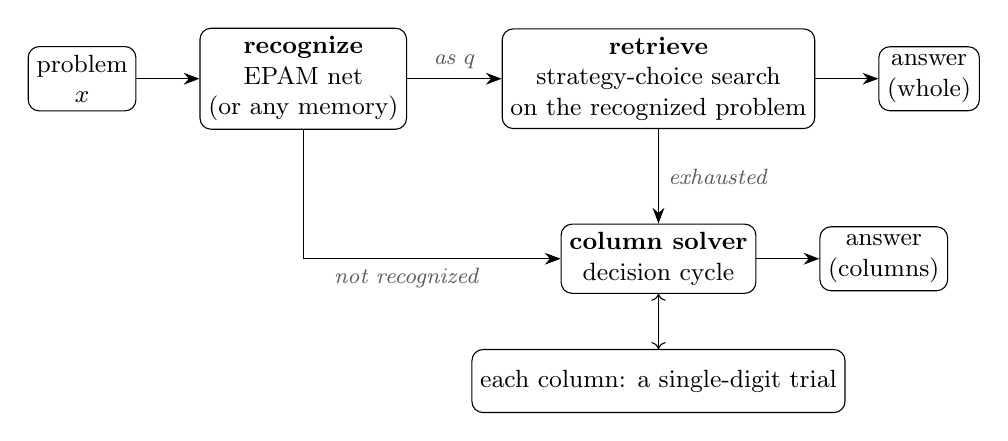
\begin{tikzpicture}[font=\small,
  box/.style={draw, rounded corners, minimum height=8mm, align=center, inner sep=3pt},
  arr/.style={-{Stealth[length=2mm]}},
  lab/.style={font=\footnotesize\itshape, text=black!65}]
  \node[box] (x) {problem\\$x$};
  \node[box, right=8mm of x] (rec) {\textbf{recognize}\\EPAM net\\(or any memory)};
  \node[box, right=12mm of rec] (ret) {\textbf{retrieve}\\strategy-choice search\\on the recognized problem};
  \node[box, right=8mm of ret] (ans) {answer\\(whole)};
  \node[box, below=12mm of ret] (sol) {\textbf{column solver}\\decision cycle};
  \node[box, right=8mm of sol] (ans2) {answer\\(columns)};
  \node[box, below=7mm of sol] (fact) {each column: a single-digit trial};
  \draw[arr] (x) -- (rec);
  \draw[arr] (rec) -- node[lab, above] {as $q$} (ret);
  \draw[arr] (ret) -- (ans);
  \draw[arr] (ret) -- node[lab, right] {exhausted} (sol);
  \draw[arr] (rec) |- node[lab, below, pos=0.7] {not recognized} (sol);
  \draw[arr] (sol) -- (ans2);
  \draw[arr, <->] (sol) -- (fact);
\end{tikzpicture}
\caption{One trial of the integrated model (\lean{MD.Integrated.itrial}).}
\label{fig:compose}
\end{figure}

\paragraph{A phenomenon, stated without a mechanism.} In the
strategy-choice model alone, a problem's errors and its backup use come
from one distribution, so errors and hesitation go together: a child
who is often wrong on a problem is also a child who often resorts to
fingers on it. Recognition can break that tie. If an unfamiliar
problem $x$ is mistaken for a familiar one $q$, the child retrieves
$q$'s answer, confidently and wrongly. CogLib states the resulting
pattern once, as a predicate over distributions of answers and the
routes that produced them
(\lean{Cog.Phenomena.ConfusionErrorPattern}):
\begin{Verbatim}[fontsize=\small]
def ConfusionErrorPattern trial retrievedWrong isRetrieved isBackup x q : Prop :=
  prob (trial q) (retrievedWrong q) = 0 ∧                             -- (i)
  prob (trial x) (retrievedWrong x) = prob (trial x) isRetrieved ∧    -- (ii)
  prob (trial x) isBackup = prob (trial q) isBackup                   -- (iii)
\end{Verbatim}
(i) The familiar $q$ is never answered wrongly by retrieval; (ii)
every retrieved answer to $x$ is wrong; (iii) $x$ backs up exactly as
often as $q$. No mechanism is named. The pattern holds for the
composition, for every encoding, net, set of strengths, criterion,
search length and backup, whenever $q$ is recognized as itself, $x$ is
recognized as $q$, $q$'s associations are \emph{sharp} (only its
correct answer clears the criterion), and the two correct answers
differ (\lean{Cog.RR.confident\_errors}; for the integrated model,
\lean{MD.Integrated.integrated\_confident\_errors}). At the
illustrative setting, a net that has learned $100+100$ and $100+200$
confuses $150+100$ with $100+100$ (\lean{MD.Example.net\_facts}) and
answers it 200 by retrieval with probability $45/46$
(\lean{MD.Example.example\_values}). Sharpness is an empirical
premise the library does not yet derive; the theorem says what follows
from it, not where it comes from.

\paragraph{The same explanation for every memory of a kind.} The theorem
just described is about EPAM's net. But what it uses of the net is
only three properties, and CogLib states them as laws against the
retriever interface, so that any memory can be asked whether it has
them: \emph{determinacy} (retrieval calls up a single item for
certain), \emph{certainty} (a studied item retrieves itself) and
\emph{stability} (studying one item leaves another's self-retrieval
unchanged). \lean{Cog.RR.confident\_errors\_of\_laws} proves the pattern
for \emph{any} memory with the three laws. EPAM's net has all three
(\lean{EPAM.determinate}, \lean{EPAM.certainty},
\lean{EPAM.stability}). A new theory of memory inherits the
explanation by proving the laws, without touching the proof. The laws
are sufficient, not shown necessary, and no claim is made that human
memory satisfies them.

\paragraph{A rival reaches the pattern another way.} ACT-R's declarative
memory, as formalized here (base-level activation, partial matching
and a retrieval threshold, at decay 1 and temperature 1;
\citealp{anderson1998})\footnote{This is a simplified ACT-R declarative
memory, and its fidelity to ACT-R is partial. With a single chunk of
weight $w$, the retrieval probability $w/(\theta+w)$ has the logistic
form ACT-R uses. With several chunks, however, retrieval failure here
competes with all the chunks inside one softmax, whereas ACT-R selects
the most active chunk under noise and then compares its activation
with the threshold. The mismatch penalty is also a multiplicative
discount in the code, $\mu^{m}$ for $m$ mismatching features, not
ACT-R's additive penalty on activation. Its values therefore do not
map onto the usual ACT-R parameter settings.} has none of the three
laws at any setting with a positive failure weight $\theta$, starting
from an empty memory (\lean{ACTR.never\_determinate},
\lean{ACTR.never\_certainty}, \lean{ACTR.never\_stability}; the
stability result also needs a nonnegative mismatch penalty and two
distinct stimuli). So the class theorem does not cover it, and at the
illustrative setting the exact pattern indeed fails
(\lean{MD.Integrated.setting\_actr\_not\_pattern}). Not covered is not
the same as cannot. A graded version of the pattern needs no
certainty: if $x$ calls up $q$, and $q$ calls up itself, each with
probability at least $1-\delta$, the pattern holds within $2\delta$
(\lean{Cog.RR.confident\_errors\_graded}). The ACT-R memory meets that
condition when $q$ is \emph{primed}: for every $\delta>0$, enough
priming suffices (\lean{Cog.RR.act\_priming\_confident\_errors}), and
having just seen $q$ is such priming, through ACT-R's own base-level
activation (\lean{Cog.RR.act\_recency\_confident\_errors}). Confident
errors therefore have two explanations in the library, from different
mechanisms: one from a memory that recognizes by discrimination, one
from a memory that is pushed toward a recently seen item.

\paragraph{The observation that would tell them apart.} Two
explanations of the same pattern invite the question of where they
differ, and here they differ on \emph{familiar} problems. EPAM's
confusions follow the features a problem shares with a stored one, and
a familiar problem is always recognized as itself, so the familiar
$100+200$ is never answered wrongly (\lean{MD.ExampleACTR.epam\_q2\_never\_wrong}).
Priming, by contrast, draws retrieval toward the primed item from
\emph{every} other item: just after seeing $100+100$ ten times, the
formalized ACT-R memory answers the stranger $150+100$ with 200 with
probability $4725/5129$, and the familiar $100+200$ with 200 with
probability $4725/6854$ (\lean{MD.ExampleACTR.recency\_values}). The
two explanations thus make opposite predictions about what priming a
familiar problem does to a child's \emph{other} familiar problems:
nothing, on one account; errors, on the other. As far as I know the
experiment has not been run. It is not hard to describe: prime one
familiar problem by repetition, then measure errors on other familiar
problems against errors on strangers. It is the kind of experimental
question that formal comparison can produce, and it came out of the
library rather than being put in.

\paragraph{Two caveats.} First, the pattern is stated over internal
routes, retrieval versus backup, not over observed responses. Applying
it to children needs a measurement interpretation of route, for
instance by latency or self-report, and infrequent backup is not the
same thing as reported confidence; each is a further bridge
(Appendix~\ref{app:bridges}). Second, the model is a demonstration of
composition, not a theory of arithmetic: carrying is error-free, the
columns are independent, and the strengths at the illustrative setting
are chosen, not fitted. The earlier edition of this introduction
\citep{coglean20261106intro} carries the multi-digit model in full,
with its further consequences and its exact values.

\subsection{Can theories be compared by what they entail? The memory theory matrix}
\label{sec:matrix}

The class theorem of the previous section needed an interface that any
memory can implement and laws stated against that interface. Once those
exist, a different kind of comparison becomes possible, and it is the
fourth demonstration. Theories of memory are usually compared by
fitting each to data, one experiment and one parameter setting at a
time, and their qualitative commitments (whether studying one item can
disturb another, whether the order of study matters, whether anything
unstudied can be retrieved) are left implicit in their
implementations. With laws stated once, any memory theory can be asked
whether it has a law, and the answer can often be proved for a whole
range of parameter settings at once. Laid out as a table of theories
by laws, the answers form a \emph{theory matrix}: a classification of
theories by what they entail, not by how well they fit.

Six laws are stated once, against the retriever interface
(\code{CogLib/CogLib/Phenomena/RetrievalLaws.lean}): certainty,
stability and determinacy, as above; \emph{order-freedom} (swapping
the last two study events leaves retrieval unchanged); \emph{recency}
(of two stimuli studied last and equally similar to the probe, the
later is retrieved more often); and \emph{stored-only} (nothing
unstudied is retrieved). Here is the first of them, to show what a law
looks like:
\begin{Verbatim}[fontsize=\small]
def Certainty (R : Retriever S Item) (s0 : S) (U : List Item) : Prop :=
  ∀ s, Reachable R s0 U s → ∀ y ∈ U, pRet R (R.study s y) y y = 1
\end{Verbatim}
In words: in any memory state reachable by studying items from the
universe $U$, studying an item $y$ and then probing with $y$ retrieves
$y$ with probability one. The laws are not independent: an order-free
memory lacks recency wherever recency can be tested
(\lean{Cog.Laws.not\_recency\_of\_orderFree}).

Four \emph{formalized families} are classified (Table~\ref{tab:matrix}):
the formalized EPAM family (discrimination nets), the formalized ACT-R
family (declarative memory, simplified as in the footnote above), the
formalized strategy-choice family (a strength memory with sampling and
a criterion) and the formalized global-matching family (after
MINERVA~2; \citealp{hintzman1984}). Each family is a narrow
formalization of one regime of its theory, with the parameters its
definitions expose, and not the theory as its authors hold it; a
verdict about a family is not a verdict about the theory. Each family
proves its own row. A verdict is read from its theorem's statement. If
the theorem binds the family's parameters, it holds at every setting:
the family \textbf{has} the law, or \textbf{never} has it. Otherwise it
is a counterexample at one setting (\emph{lacks}). A generator builds
the table from the theorems, checks that names agree with statements,
and checks each cell's axioms. Every law holds for some family and
fails for another, and no two families share a row.

\begin{table}[H]
\centering\footnotesize\setlength{\tabcolsep}{4pt}
\begin{tabularx}{\linewidth}{@{}>{\raggedright\arraybackslash}p{0.22\linewidth}*{6}{>{\centering\arraybackslash}X}@{}}
\toprule
Formalized family & Certainty & Stability & Order-free & Recency & Stored only & Determinate \\
\midrule
EPAM & \textbf{has} & \textbf{has} & lacks & lacks & \textbf{has} & \textbf{has} \\
ACT-R & \textbf{never} & \textbf{never} & \textbf{never} & \textbf{has} & \textbf{has} & \textbf{never} \\
Strategy choice & lacks & lacks & \textbf{has} & \textbf{never} & \textbf{has} & lacks \\
Global matching & lacks & lacks & \textbf{has} & \textbf{never} & lacks & \textbf{has} \\
\midrule
\emph{Adopted interpretation of the evidence} & \emph{lacks} & \emph{mixed} & \emph{lacks} & \emph{has} & \emph{mixed} & \emph{mixed} \\
\bottomrule
\end{tabularx}
\caption{The memory theory matrix. Each row is a formalized family, a narrow formalization of one regime of the named theory, not the theory itself. Above the line, each verdict is a theorem; \textbf{has} and \textbf{never} hold across the range of parameters and stimuli each theorem states (for ACT-R, a positive failure weight $\theta$, a nonnegative mismatch penalty $\mu$, positive for recency, an empty starting memory, and two distinct stimuli where a law compares them), and lacks is a counterexample at one setting. The last row is not a theorem but an illustrative interpretation of the evidence about people, with sources and bridges (\code{notes/evidence.json}). The theorems are in \code{EPAM/EPAM/Laws.lean}, \code{ACTR/ACTR/Laws.lean}, \code{StrategyChoice/StrategyChoice/Laws.lean} and \code{GlobalMatching/GlobalMatching/Laws.lean}.}
\label{tab:matrix}
\end{table}

The last row records, outside Lean, one interpretation of what
experiments show about people. It is illustrative: it shows how
evidence attaches to laws, not which theory is right. Each judgment
rests on a bridge from what an experiment measures (reports,
decisions) to what a law concerns (what memory retrieves), and the
bridges are not formalized (Appendix~\ref{app:bridges}). Some are
weak. Certainty concerns probing with a stimulus just after studying
it; that cued recall retrieves words free recall missed
\citep{tulving1966} bears on it only indirectly. Recency is a strict
comparison between the last two, equally similar stimuli;
serial-position effects \citep{murdock1962,glanzer1966} are averages
over lists. Stability \citep{mcgeoch1932,barnes1959,ratcliff1990},
stored-only retrieval \citep{posner1968,roediger1995} and determinacy
are recorded as mixed. A family would be incompatible with the
interpretation of a law when its verdict holds at every setting and
the judgment goes the other way.

The formal verdicts are the result: four formalized families
classified against six laws, each verdict proved. Reading them against
people is a further step, only as good as the bridges, and no
conclusion about which theory of memory is right is drawn here. What
the matrix does is make such questions precise and extensible: a new
memory adds a row, a new law a column, a better bridge can replace a
weak one, and disagreeing with a judgment is a precise act with
traceable consequences.

\section{Discussion}
\label{sec:disc}

The four demonstrations answer four different questions, but they
share one shape, and the shape is the point of CogLean. In each,
something was stated once, apart from any particular theory: a
phenomenon of verification, a pattern of confident errors, a law of
retrieval. Then one or more theories, each written as a mechanism,
were held to it, and what each entails was proved rather than argued
or sampled. The strategy-choice chapter was held to its own claims;
two models of semantic memory were held to three phenomena; three
theories were composed and the composition held to a pattern that
none of them produces alone, after which a fourth theory was held to
the same pattern; and four memories were held to six laws. Two of the
four did what the introduction promised first: they wrote down what
we already believed, precisely, and established its exact scope. That
Collins and Quillian's network cannot show typicality was folklore;
now it is a theorem about every network. The other two went further
and found things that were not known: a condition missing from a
published claim, and a prediction on which two explanations of the
same pattern disagree. Neither result is about children directly.
Each is about a theory, and what it means for children depends on the
bridges of Appendix~\ref{app:bridges}. That distinction is not a
weakness. It is what lets the results be stated exactly and
contested precisely. Because the phenomena and laws are shared, each result is available to the next
theory that uses the same constructs, and the explanations themselves
become reusable objects. A theorem characterizes a class of
mechanisms; another theory joins the class by proving its laws, or
reaches the same phenomenon by a different route; and the resulting
explanations can be compared, composed and challenged.

CogLean's targets are \emph{phenomena}, regularities of behavior stated
without mechanisms; observed, a phenomenon is a psychological fact,
and derived but unobserved, a prediction. Its central theorems are
meant as \emph{explanations}: deductions of a phenomenon from
mechanisms and stated assumptions \citep{hempel1948}, carried through
the operation of mechanisms \citep{machamer2000}. Not every valid
proof explains \citep{steiner1978}; which theorems explain is a
judgment the library records openly. A phenomenon stated over internal
routes, like the confusion-error pattern, is a computational property
until a measurement interpretation connects those routes to behavior
(Appendix~\ref{app:bridges}).

Proof, experiment and simulation can each expose the limits of the
others. Lean checks that conclusions follow from premises. Whether
premises hold of people is for experiment, and whether a theorem's
conditions arise when a model runs is for simulation. An independent
simulation of the multi-digit model found valid theorems whose
hypotheses were never realized in its learning histories
\citep{coglean}. Every theorem in CogLean is \emph{valid}: Lean has
checked that its conclusion follows from its premises. That guarantee
is the foundation of everything else, but it is not enough. Validity
is neither empirical adequacy, whether the premises hold of people,
nor explanation. A theorem whose premises simply restate its
phenomenon is valid but empty, so the repository records, for each
headline result, how far it lies from its premises. What separates
explanation from restatement is often a second consequence of the same
mechanism, as when the EPAM and ACT-R explanations of confident errors
differ on familiar problems.

CogLean is not the first formalization of cognitive theory. Soar was
specified in Z \citep{milnes1992}; Sceptic is an executable
specification language for cognitive models \citep{cooper1996}; ACT-R
was reconstructed to separate its commitments from its implementation
\citep{stewart2007}, given an operational semantics with a provably
correct translation \citep{gall2018,gall2017confluence}, and
translated to timed automata for exhaustive analysis
\citep{langenfeld2019,langenfeld2021}; a common formal ground for
architectures has been proposed \citep{ragni2018}; Soar models have
been compiled for probabilistic model checking
\citep{ganeriwala2026,kwiatkowska2011}; verbal theories have been
formalized as logic programs and automata \citep{rohner2021,finkel2025};
and critical tests of ACT-R have been derived from its core
assumptions \citep{fisher2025}. Each of these brought formal rigor to
one theory, and several went much further than CogLean in their own
direction. CogLean differs in three ways. The model and the formal
object are the same thing: the definition that runs is the definition
the theorems are about. Its theorems hold for classes rather than
instances: a model checker analyzes one specified model exhaustively,
even with symbolic parameters \citep{hahn2011}, whereas a CogLean
theorem covers every mechanism satisfying stated laws. And it works
across theories rather than within one, and is meant to be cumulative,
a library that others extend, as Mathlib is, rather than a
formalization that lives in a single paper. These are differences of
kind, not of scale, and they come at a cost: model checking can verify
large, detailed models that would be laborious to reason about
deductively, Gall's semantics of ACT-R is far more faithful to ACT-R
than the simplified memory used here, and CogLean's models are small.
A model checker can tell us what a particular model does; a theorem
tells us what every model of a kind must do.

The framework does not establish psychological plausibility. Key
conditions, such as sharp associations, are assumed, not derived, and
the examples' parameters are chosen, not learned. Exact rationals
restrict some theories to special cases: the ACT-R memory appears at
decay 1 and temperature 1. Exact finite distributions will not scale
to continuous or neural models without other mathematics. And the
bridges from what the theorems concern to what experiments measure are
stated, not formalized.

\section{An invitation}
\label{sec:invite}

Newell asked how cognitive science could become cumulative. CogLean is
not a theory of cognition, and it is not meant to be a collection of
independently formalized models. It is meant to become what Mathlib is
for mathematics: a cumulative library of mechanisms, phenomena, laws
and explanations, in which each contribution enables further
deductions, and in which complex models stay aligned with equally
complex explanations of their behavior as the library grows and
changes. In such a library researchers with different commitments can
state, compare, criticize and improve explanations, and disagreements
about assumptions, mechanisms, evidence and predictions become
explicit objects of study. Cognitive science can then accumulate not
only experiments and models, but also what can be established about
the relationships among theories and phenomena, and can reason its way
to things it did not previously know.

The demonstrations suggest what different kinds of cognitive
scientists could contribute, and most of it needs no Lean.
Experimentalists could contribute phenomena: a regularity stated
precisely enough to become a target, like the three phenomena of
verification, is a contribution in itself, and so is a judgment about
the evidence, like the last row of the matrix, or a test of a
prediction the library has produced, like the priming experiment of
Section~\ref{sec:compose}. Modelers could contribute mechanisms, and
could challenge the representations the existing ones assume; a
theory enters the library by stating its postulates as choices of
CogLib constructs, as the strategy-choice model does, and a reader who
thinks a postulate has been misread can say which. Mathematical
psychologists could contribute laws and class theorems: the matrix has
four rows and six columns, and both are open. Methodologists could
contribute bridges, the assumptions that connect what a theorem
concerns to what an experiment measures, which this paper leaves
informal and which are themselves pieces of psychological theory.
And researchers in formal methods could contribute abstractions,
proofs and tooling, including ways to make all of this easier for
everyone else. As AI systems get better at proofs, separating the
social work of proposing, contesting and interpreting theories from
the mechanical checking of their consequences may matter more, and
much of the Lean in this repository was in fact written that way.

This paper has followed one path through CogLean. It is only one of
many, and I hope that others will take CogLean in directions of their
own.

\section{Availability}

Everything in this paper is open source and available in
CogLean-Intro \citep{cogleanintro}, a small,
self-contained edition of the library; the earlier edition
\citep{coglean20261106intro} carries the multi-digit model in full,
and the CogLean repository \citep{coglean} holds the wider library.
Every theorem is fully proved, with no \code{sorry}, and depends only
on Lean's standard axioms.

\section{Acknowledgements}

The CogLean concept grew out of conversations between Chris Bates,
Pete Pirolli, and the author. Bates and Pirolli, as well as John Laird
and Christian Lebiere provided useful early guidance. Almost all of the
Lean programming in the CogLean project was accomplished by Claude
Code (mostly Opus 5.5) with extensive guidance from the author, as
well as ongoing feedback from ChatGPT as well as various cognitive
scientists including those named above. Papers and presentations were
initially drafted by LLMs and then substantially rewritten by the
author. Any remaining errors, including hallucinations, are the
author's alone.

\bibliographystyle{unsrtnat}
\bibliography{refs}

\clearpage
\appendix
\section{From computational properties to psychological phenomena: bridges}
\label{app:bridges}

A theorem about a model establishes that the model and its assumptions, $M$, entail a computational property $P$. Explaining what people do takes two further steps. An observation bridge, $B$, connects $P$ to a prediction about measurable behavior; an empirical test then compares that prediction with data:
\[
\underbrace{M \Rightarrow P}_{\text{computational deduction}}
\qquad
\underbrace{P + B \Rightarrow O_{\text{predicted}}}_{\text{observation bridge}}
\qquad
\underbrace{O_{\text{predicted}}\ \text{vs.}\ O_{\text{measured}}}_{\text{empirical test}}
\]
Lean checks the first step and can check the second when the bridge is formalized; the third is empirical science. A valid bridge can connect a valid theorem to a prediction that people do not exhibit. The explanation is then empirically inadequate, although every deduction in it is correct.

Two quite different things can be called bridges. An \emph{implementation bridge} relates two formal descriptions; the multi-digit model has one, the equivalence of the column solver and direct column arithmetic (\lean{MD.Solver.bridge}), and Lean proves it from the definitions. An \emph{observation bridge} relates a formal description to measurements. It cannot be proved from definitions, because one side is a claim about people. In the body of the paper, ``bridge'' means an observation bridge.

The confusion-error pattern (Section~\ref{sec:compose}) names no mechanism, but it is stated over internal routes, retrieval and backup. A child's behavior shows an answer, perhaps a response time, perhaps a confidence report, but not the route. Reaching behavior takes assumptions such as these: retrieval is usually fast; backup is usually slower; fast answers given with high confidence usually come from retrieval. With a model of latency and confidence built on them, one could derive an observable prediction: the confused problem yields more fast, confident errors than the familiar one. The prediction is conditional on the bridge, and the bridge may be false. Theory-neutral and observable are different properties of a phenomenon. The verification phenomena of Section~\ref{sec:cq} are closer to observation, since cost is ordinal and the data are response times, but ``cost'' and ``time'' are still joined by an assumption.

The matrix's evidence row works the same way. Certainty is a precisely defined law: just after an item is studied, probing memory with that item retrieves it for certain. Cued recall recovers words that free recall missed \citep{tulving1966}. Does that contradict certainty? Not necessarily, since neither free nor cued recall is the operation the law describes. Counting the experiment as evidence against the law needs a bridge from the experimental conditions to that operation, and the one recorded in \code{notes/evidence.json} is weak. None of this weakens the theorems. It locates the further scientific work their empirical reading needs.

An observation bridge is itself a piece of psychological theory, not a translation of terminology: that fast responses reflect retrieval is a substantive hypothesis about cognition. Bridges can therefore be proposed, criticized, compared and tested, and they could be formalized: an observation model, conceptually \code{observe : Internal} $\to$ \code{Dist Observable}, would map each internal outcome to a distribution over answers, times and reports, and Lean could then check that a mechanism and an observation model together entail an observable phenomenon. It could not check that the observation model describes people. CogLean does not close the gap between computational models and psychological observations. It makes the gap explicit, lets proposed bridges be stated precisely, and lets their deductive consequences be checked.

\section{Glossary}
\label{app:glossary}

The terms below are defined where the paper first uses them; this appendix collects them for reference. Table~\ref{tab:map} maps CogLean's constructs onto familiar scientific notions.

\begin{table}[h]
\centering\small
\begin{tabularx}{\linewidth}{@{}>{\raggedright\arraybackslash}p{0.27\linewidth}>{\raggedright\arraybackslash}X@{}}
\toprule
Scientific notion & In CogLean \\
\midrule
Model (the program) & executable definitions: the same ones that run \\
Mechanism (postulate) & a CogLib process, chosen by a theory and cited to its source \\
Phenomenon & a predicate over a task's outcomes, with no mechanism: a target \\
Psychological fact & a phenomenon judged to hold of people: outside Lean, recorded with sources \\
Prediction & a theorem's conclusion about an unobserved phenomenon \\
Assumption & a condition (a theorem's hypothesis) or a law (a property of a mechanism) \\
Explanation & a theorem and its lemmas: mechanisms and assumptions entail the phenomenon \\
Deduction & what Lean's kernel checks \\
Witness & a value computed at one setting: not an explanation \\
\bottomrule
\end{tabularx}
\caption{Scientific notions and what they are in CogLean.}
\label{tab:map}
\end{table}

\subsection*{Lean}
\begin{description}[leftmargin=1em,itemsep=1pt,font=\normalfont\itshape]
\item[Lean.] A functional programming language that is also a proof assistant. A definition is both a program that runs and a mathematical object that theorems are about.
\item[Kernel.] The small part of Lean that checks every proof. Deduction, in CogLean, is what the kernel checks.
\item[\code{sorry}.] Lean's placeholder for a missing proof. No CogLean theorem uses it.
\item[Standard axioms.] \code{propext}, \code{Quot.sound} and \code{Classical.choice}, the only axioms CogLean's theorems depend on. A law is never an axiom; it is a hypothesis.
\item[Fully qualified name.] A declaration's full name, which says where to find it: \texttt{Cog.} for CogLib; \texttt{SC.} (strategy choice), \texttt{SemanticMemory.}, \texttt{EPAM.}, \texttt{ACTR.} and \texttt{GM.} (global matching) for the theories; \texttt{MD.} for the multi-digit model.
\item[Exact rationals.] Probabilities are fractions (Lean's \code{Rat}), not floating-point numbers, so values at a setting are computed and checked exactly.
\item[Mathlib.] Lean's community library of mathematics, the model for CogLib.
\end{description}

\subsection*{CogLean}
\begin{description}[leftmargin=1em,itemsep=1pt,font=\normalfont\itshape]
\item[CogLean.] The project of applying Lean in cognitive science.
\item[CogLib.] The shared library: representations, memories, processes, the retriever interface, and theory-neutral phenomena and laws with their theorems. Nothing in it depends on any particular theory.
\item[Theory.] A package that states its postulates as choices of CogLib constructs, cites its sources, and proves its phenomena and its mechanisms' laws.
\item[Application.] A task model built from theories and library mechanisms, such as the multi-digit model.
\item[Mechanism.] A definition of a process, such as how a net sorts a code. A theory's postulate is a choice of mechanism.
\item[Distribution.] An exact finite probability distribution over outcomes (\lean{Cog.Dist}).
\item[Retriever.] The interface any memory can implement (\lean{Cog.Retriever}): study an item; retrieve a distribution over stored items.
\item[Verifier.] The interface any model of sentence verification can implement (\lean{Cog.Verifier}): for ``x is a c'', a truth value and an ordinal cost.
\item[Phenomenon.] A predicate over a task's outcomes, with no mechanism in it: a target. Observed, it is a psychological fact; derived but unobserved, a prediction. One stated over internal routes is a computational property until a measurement interpretation connects the routes to behavior.
\item[Law.] A property of a mechanism, stated against an interface, such as certainty. It is a hypothesis of the theorems that use it.
\item[Condition.] A theorem's hypothesis: situational, an unexplained empirical premise, or well-formedness.
\item[Explanation.] A theorem and its lemmas, showing that mechanisms and assumptions entail a phenomenon. Not every valid proof explains.
\item[Class theorem.] A theorem for every mechanism that satisfies stated laws, such as \lean{Cog.RR.confident\_errors\_of\_laws}.
\item[Graded.] Holding within a tolerance $\delta$ rather than exactly.
\item[Setting.] A choice of parameter values.
\item[Witness.] A value computed at one setting. It shows that hypotheses can be met and that models diverge, but not why; it is not an explanation.
\item[Verdict.] A matrix cell, read from its theorem's statement: \textbf{has} or \textbf{never} (at every setting), or \emph{lacks} (a counterexample at one setting).
\item[Formalized family.] A narrow formalization of one regime of a theory, with the parameters its definitions expose; a row of the matrix. It is not the theory itself.
\item[Bridge.] The link from what an experiment measures to what a law or phenomenon concerns. A scientific assumption, not formalized here (Appendix~\ref{app:bridges}).
\item[Interpretation of the evidence.] The matrix's last row: one illustrative, contestable reading of experiments about people, with sources and bridges (\code{notes/evidence.json}).
\end{description}

\subsection*{Phenomena and laws}
\begin{description}[leftmargin=1em,itemsep=1pt,font=\normalfont\itshape]
\item[Distance effect.] Of two true statements about one instance, the one whose category is farther up the hierarchy costs more.
\item[Typicality effect.] Two instances equally far below a category, both verified true, at different costs.
\item[Reversal.] An instance verified faster as a member of a farther category than of a nearer one.
\item[Confusion-error pattern.] A familiar problem $q$ is never answered wrongly by retrieval, every retrieved answer to a problem $x$ is wrong, and $x$ backs up exactly as often as $q$ (\lean{Cog.Phenomena.ConfusionErrorPattern}).
\item[Certainty.] Just after a stimulus is studied, probing with it retrieves it for certain.
\item[Stability.] Studying one stimulus leaves the chance that another retrieves itself unchanged.
\item[Determinacy.] Retrieval calls up a single item for certain.
\item[Order-freedom.] Swapping the last two study events leaves retrieval unchanged.
\item[Recency.] Of two stimuli studied last and equally similar to the probe, the later is retrieved more often.
\item[Stored-only.] Nothing unstudied is retrieved.
\end{description}

\subsection*{The cognitive models}
\begin{description}[leftmargin=1em,itemsep=1pt,font=\normalfont\itshape]
\item[Strategy choice (DOA).] Siegler and Shrager's distributions of associations \citep{siegler1984}. Each problem is associated with answers, with varying strengths. A search samples an answer in proportion to strength and states it if its strength clears a \emph{confidence criterion}, for up to $n$ searches (the \emph{search length}); otherwise a backup strategy (fingers, then counting) is used. Its memory, sampling by strength with a criterion, is the matrix's strength family.
\item[Sharp.] A problem's associations are sharp when only its correct answer clears the criterion.
\item[Hierarchical network.] Collins and Quillian's model \citep{collins1969}: concepts in a hierarchy, properties stored at the highest node they apply to, verification by climbing.
\item[Feature comparison.] Smith, Shoben and Rips's model \citep{smith1974}: meanings as feature sets, a first stage on overall similarity, a second on defining features.
\item[EPAM.] Recognition by a discrimination net \citep{feigenbaum1962}. A stimulus's code, a vector of features, is sorted down the net's tests to a stored \emph{image}; when a stimulus is confused with a stored one, learning adds a test on the first feature where they differ.
\item[Column solver.] The backup in the multi-digit model: column-by-column addition on CogLib's decision cycle, with impasses and repairs \citep{brown1980}, each column a strategy-choice trial.
\item[ACT-R declarative memory.] Retrieval by base-level activation (recency and frequency of study), partial matching and a retrieval threshold \citep{anderson1998}; formalized here at decay 1 and temperature 1. \emph{Priming} raises an item's activation.
\item[Global matching.] A memory after MINERVA~2 \citep{hintzman1984}, in which a probe is compared with every stored trace at once.
\item[Recognize, retrieve, else back up.] CogLib's general composition (\lean{Cog.recognizeRetrieve}): recognize the stimulus, retrieve an answer from what it is recognized as, and back up if nothing is recognized or retrieval fails.
\item[Route.] Whether an answer came from retrieval or from the backup.
\item[$x$ and $q$.] A problem and the familiar problem it is taken for, as $150+100$ and $100+100$.
\end{description}

\end{document}
